\documentclass[10pt]{extarticle}

\usepackage[english]{babel}
\usepackage{graphicx}
\usepackage{framed}
\usepackage[normalem]{ulem}
\usepackage{indentfirst}
\usepackage{amsmath,amsthm,amssymb,amsfonts}
\usepackage{mathtools} % Wraparound amsmath. For fancy math typesetting
\usepackage[nointegrals]{wasysym} % nointegrals prevents wasysym from overwriting integral symbols from LaTeX and amsmath
\usepackage{bbm} % For extended bold and blackboard bold characters
\usepackage[italicdiff]{physics} % italicdiff causes derivatives to be rendered with italic d's instead of upright d's
\usepackage[T1]{fontenc}
\usepackage{xparse}
\usepackage{xstring}
% \usepackage{pifont} % For unusual symbols
% \usepackage{mathdots} % For unusual combinations of dots
\usepackage{wrapfig}
\usepackage{lmodern,mathrsfs}
\usepackage[inline,shortlabels]{enumitem}
\setlist{topsep=2pt,itemsep=2pt,parsep=0pt,partopsep=0pt}
\usepackage[table,dvipsnames]{xcolor}
\usepackage[utf8]{inputenc}
\usepackage{csquotes} % Must be loaded AFTER inputenc
\usepackage[a4paper,top=0.5in,bottom=0.2in,left=0.5in,right=0.5in,footskip=0.3in,includefoot]{geometry}
\usepackage[most]{tcolorbox}
\usepackage{tikz,tikz-3dplot,tikz-cd,tkz-tab,tkz-euclide,pgf,pgfplots}
\pgfplotsset{compat=newest}
% \usepackage{comment} % For commenting large blocks of text and math efficiently
% \usepackage{fancyvrb} % For custom verbatim environments
\usepackage{multicol}
\usepackage[bottom,multiple]{footmisc} % Ensures footnotes are at the bottom of the page, and separates footnotes by a comma if they are adjacent
\usepackage[backend=bibtex,style=numeric]{biblatex}
\renewcommand*{\finalnamedelim}{\addcomma\addspace} % Forces authors' names to be separated by comma, instead of "and"
\addbibresource{bibliography}
\usepackage[colorlinks,linkcolor=.,citecolor=blue,urlcolor=violet]{hyperref}
\usepackage[nameinlink]{cleveref} % nameinlink ensures that the entire element is clickable in the pdf, not just the number

\newcommand{\remind}[1]{\textcolor{red}{\textbf{#1}}} % To remind me of unfinished work to fix later
\newcommand{\hide}[1]{} % To hide large blocks of code without using % symbols

% Same as \href, but the text appears in typewriter font and in a custom color
\newcommand{\Href}[3][red!50!black]{\href{#2}{\textcolor{#1}{\texttt{#3}}}}

\newcommand{\ep}{\varepsilon}
\newcommand{\vp}{\varphi}
\newcommand{\lam}{\lambda}
\newcommand{\Lam}{\Lambda}
\DeclareDocumentCommand\ip{ l m }{\braces#1{\langle}{\rangle}{#2}} % Inner product ⟨x,y⟩ (but only one argument is taken, so \ip{x,y} renders as ⟨x,y⟩)
\DeclareDocumentCommand\floor{ l m }{\braces#1{\lfloor}{\rfloor}{#2}} % Floor function ⌊x⌋
\DeclareDocumentCommand\ceil{ l m }{\braces#1{\lceil}{\rceil}{#2}} % Ceiling function ⌈x⌉

% Shortcuts for blackboard bold letters, e.g. \A outputs \mathbb{A}
\def\do#1{\csdef{#1}{\mathbb{#1}}}
\docsvlist{A,B,C,D,E,F,G,I,J,K,M,N,Q,R,T,U,V,W,X,Y,Z}
% \H is already defined as a 1-argument command, it places a double acute accent (hungarumlaut) on a character, e.g. \H{o} yields ő
% \L is already defined as the uppercase Ł (L with stroke)
% \O is already defined as the uppercase Ø (O with stroke)
% \P is already defined as the pilcrow ¶ (paragraph mark)
% \S is already defined as the section sign §

% Shortcuts for calligraphic letters, e.g. \As outputs \mathcal{A}
\def\do#1{\csdef{#1s}{\mathcal{#1}}}
\docsvlist{A,B,C,D,E,F,G,H,I,J,K,L,M,N,O,P,Q,R,S,T,U,V,W,X,Y,Z}

% Shortcuts for letters with a bar on top, e.g. \Abar outputs \overline{A}
\def\do#1{\csdef{#1bar}{\overline{#1}}}
\docsvlist{a,b,c,d,e,f,g,i,j,k,l,m,n,o,p,q,r,s,t,u,v,w,x,y,z,A,B,C,D,E,F,G,H,I,J,K,L,M,N,O,P,Q,R,S,T,U,V,W,X,Y,Z}
% \hbar is already defined as the symbol ℏ (reduced Planck constant)

% Shortcuts for boldface letters, e.g. \Ab outputs \textbf{A}
\def\do#1{\csdef{#1b}{\textbf{#1}}}
\docsvlist{a,b,c,d,e,f,g,h,i,j,k,l,m,n,o,q,r,t,u,w,x,y,z,A,B,C,D,E,F,G,H,I,J,K,L,M,N,O,P,Q,R,S,T,U,V,W,X,Y,Z}
% \pb is already defined (by the physics package) as a 2-argument command, denoting the anticommutator or Poisson bracket, e.g. \pb{A,B} yields {A,B}
% \sb is already defined in the LaTeX kernel. This is a fundamental LaTeX command, DO NOT overwrite it!
% \vb is already defined (by the physics package) as a 1-argument command, for boldface text, e.g. \vb{A} yields \textbf{A}

% Shortcuts for letters with a tilde on top, e.g. \Atil outputs \widetilde{A}
\def\do#1{\csdef{#1til}{\widetilde{#1}}}
\docsvlist{a,b,c,d,e,f,g,h,i,j,k,l,m,n,o,p,q,r,s,t,u,v,w,x,y,z,A,B,C,D,E,F,G,H,I,J,K,L,M,N,O,P,Q,R,S,T,U,V,W,X,Y,Z}

\newcommand{\tm}{^{\mathsf{T}}}     % Transpose
\newcommand{\hm}{^{\mathsf{H}}}     % Conjugate transpose (Hermitian conjugate)
\newcommand{\itm}{^{-\mathsf{T}}}   % Inverse transpose
\newcommand{\ihm}{^{-\mathsf{H}}}   % Inverse conjugate transpose (Inverse Hermitian conjugate)
\newcommand{\ex}{\textbf{e}_x}
\newcommand{\ey}{\textbf{e}_y}
\newcommand{\ez}{\textbf{e}_z}
\newcommand{\Aint}{A^\circ}
\newcommand{\Bint}{B^\circ}
\newcommand{\limk}{\lim_{k\to\infty}}
\newcommand{\limm}{\lim_{m\to\infty}}
\newcommand{\limn}{\lim_{n\to\infty}}
\newcommand{\limx}[1][a]{\lim_{x\to#1}}
\newcommand{\limz}[1][{z_0}]{\lim_{z\to#1}}
\newcommand{\liminfm}{\liminf_{m\to\infty}}
\newcommand{\limsupm}{\limsup_{m\to\infty}}
\newcommand{\liminfn}{\liminf_{n\to\infty}}
\newcommand{\limsupn}{\limsup_{n\to\infty}}
\newcommand{\sumkn}{\sum_{k=1}^n}
\newcommand{\sumk}[1][1]{\sum_{k=#1}^\infty}
\newcommand{\summ}[1][1]{\sum_{m=#1}^\infty}
\newcommand{\sumn}[1][1]{\sum_{n=#1}^\infty}
\newcommand{\emp}{\varnothing}
\newcommand{\exc}{\backslash}
\newcommand{\sub}{\subseteq}
\newcommand{\sups}{\supseteq}
\newcommand{\capp}{\bigcap}
\newcommand{\cupp}{\bigcup}
\newcommand{\kupp}{\bigsqcup}
\newcommand{\cappkn}{\bigcap_{k=1}^n}
\newcommand{\cuppkn}{\bigcup_{k=1}^n}
\newcommand{\kuppkn}{\bigsqcup_{k=1}^n}
\newcommand{\cappk}[1][1]{\bigcap_{k=#1}^\infty}
\newcommand{\cuppk}[1][1]{\bigcup_{k=#1}^\infty}
\newcommand{\cappm}[1][1]{\bigcap_{m=#1}^\infty}
\newcommand{\cuppm}[1][1]{\bigcup_{m=#1}^\infty}
\newcommand{\cappn}[1][1]{\bigcap_{n=#1}^\infty}
\newcommand{\cuppn}[1][1]{\bigcup_{n=#1}^\infty}
\newcommand{\kuppk}[1][1]{\bigsqcup_{k=#1}^\infty}
\newcommand{\kuppm}[1][1]{\bigsqcup_{m=#1}^\infty}
\newcommand{\kuppn}[1][1]{\bigsqcup_{n=#1}^\infty}
\newcommand{\cappa}{\bigcap_{\alpha\in I}}
\newcommand{\cuppa}{\bigcup_{\alpha\in I}}
\newcommand{\kuppa}{\bigsqcup_{\alpha\in I}}
\newcommand{\dx}{\,dx}
\newcommand{\dy}{\,dy}
\newcommand{\dt}{\,dt}
\newcommand{\dmu}{\,d\mu}
\newcommand{\dnu}{\,d\nu}
\DeclareMathOperator{\glb}{\text{glb}}
\DeclareMathOperator{\lub}{\text{lub}}
\newcommand{\xh}{\widehat{x}}
\newcommand{\yh}{\widehat{y}}
\newcommand{\zh}{\widehat{z}}
\newcommand{\<}{\langle}
\renewcommand{\>}{\rangle}
\newcommand\todo[1]{\textcolor{red}{#1}}

\newcommand{\figuresvisualizationpath}{D:/projecten/syntra/git-repos/data-science-syntra-ab/04 data visualizatie/figures}

% Shortcuts for inverse hyperbolic functions (and other operators with the same structure)
\def\do#1{\csdef{#1}{\trigbraces{\operatorname{#1}}}}
\docsvlist{
    asinh,acosh,atanh,acoth,asech,acsch,
    arsinh,arcosh,artanh,arcoth,arsech,arcsch,
    arcsinh,arccosh,arctanh,arccoth,arcsech,arccsch,
    sen,tg,cth,senh,tgh,ctgh,
    Re,Im,arg,Arg,im,ker
}

% \spn has to be defined separately as the syntax "spn" is different from the output "span"
% \span is already defined in the LaTeX kernel. This is a fundamental LaTeX command, DO NOT overwrite it!
\newcommand{\spn}{\trigbraces{\operatorname{span}}}

\makeatletter
% Redefining the commands \iff (given by LaTeX), \implies and \impliedby (given by amsmath)
% Math mode is automatically enforced, starred version makes the arrows shorter
\renewcommand{\impliedby}{\@ifstar{\ensuremath{\Longleftarrow}}{\ensuremath{\Leftarrow}}} % Corresponding Unicode character: U+21D0 ⇐
\renewcommand{\implies}{\@ifstar{\ensuremath{\Longrightarrow}}{\ensuremath{\Rightarrow}}} % Corresponding Unicode character: U+21D2 ⇒
\renewcommand{\iff}{\@ifstar{\ensuremath{\Longleftrightarrow}}{\ensuremath{\Leftrightarrow}}} % Corresponding Unicode character: U+21D4 ⇔
\makeatother

\newtheoremstyle{mystyle}{}{}{}{}{\sffamily\bfseries}{.}{ }{}
\makeatletter
\renewenvironment{proof}[1][\proofname] {\par\pushQED{\qed}{\normalfont\sffamily\bfseries\topsep6\p@\@plus6\p@\relax #1\@addpunct{.} }}{\popQED\endtrivlist\@endpefalse}
\makeatother
% \renewcommand{\qedsymbol}{\coolqed{0.32}} % Implements the new QED symbol
\theoremstyle{mystyle}{\newtheorem*{remark}{Remark}}
\theoremstyle{mystyle}{\newtheorem*{remarks}{Remarks}}
\theoremstyle{mystyle}{\newtheorem*{example}{Example}}
\theoremstyle{mystyle}{\newtheorem*{examples}{Examples}}
\theoremstyle{definition}{\newtheorem*{exercise}{Exercise}}

% Warning environment
\newtheoremstyle{warn}{}{}{}{}{\normalfont}{}{ }{}
\theoremstyle{warn}
\newtheorem*{warning}{\warningsign{0.2}\relax}

% Symbol for the warning environment, designed to be easily scalable
\newcommand{\warningsign}[1]{
    \tikz[scale=#1,every node/.style={transform shape}]{
        \draw[-,line width={#1*0.8mm},red,fill=yellow,rounded corners={#1*2.5mm}] (0,0)--(1,{-sqrt(3)})--(-1,{-sqrt(3)})--cycle;
        \node at (0,-1) {\fontsize{48}{60}\selectfont\bfseries!};
}}

% \newcommand{\coolqed}[1]{\includegraphics[width=#1cm]{sunglasses_emoji.png}} % QED symbol

% verbbox environment, for showing verbatim text next to code output (for package documentation and user learning purposes)
\NewTCBListing{verbbox}{ !O{} }{boxrule=1pt,sidebyside,skin=bicolor,colback=gray!10,colbacklower=white,valign=center,top=2pt,bottom=2pt,left=2pt,right=2pt,#1} % Last argument allows more tcolorbox options to be added

\NewDocumentCommand{\solidball}{ s O{} m O{white} m }{
\tikz[scale=#5,every node/.style={transform shape}]{
    \shade[ball color=#3] (0,0) circle (0.5); %solid ball with no label
    \IfBooleanF{#1}{
        \clip (0,0) circle (0.25);
        \shade[ball color=#4] (0,0) circle (0.5);
    }
    \node[font=\sffamily\bfseries\selectfont] at (0,0) {#2}; % Label
}
}

\NewDocumentCommand{\stripedball}{ s O{} m O{white} m }{
\tikz[scale=#5,every node/.style={transform shape}]{
    \shade[ball color=#4] (0,0) circle (0.5);
    \clip (-0.5,-0.35) rectangle (0.5,0.35);
    \shade[ball color=#3] (0,0) circle (0.5);
    \IfBooleanF{#1}{
        \clip (0,0) circle (0.25);
        \shade[ball color=#4] (0,0) circle (0.5);
    }
    \node[font=\sffamily\bfseries\selectfont] at (0,0) {#2}; % Label
}
}

% Official colors for Aramith Tournament pool balls
% Colors taken from https://www.aramith.com/story-behind-aramith-tournament-black-colours
\definecolor{aramith_color_0}{HTML}{FFFFDF} % Cue ball and secondary color for all balls
\definecolor{aramith_color_1}{HTML}{FFD501} % 1 and 9
\definecolor{aramith_color_2}{HTML}{013CB1} % 2 and 10
\definecolor{aramith_color_3}{HTML}{E71C01} % 3 and 11
\definecolor{aramith_color_4}{HTML}{4F029C} % 4 and 12
\definecolor{aramith_color_5}{HTML}{FA4D00} % 5 and 13
\definecolor{aramith_color_6}{HTML}{0E5D01} % 6 and 14
\definecolor{aramith_color_7}{HTML}{6D071A} % 7 and 15
\definecolor{aramith_color_8}{HTML}{000000} % 8 (black)


\makeatletter
% Adapted from https://tex.stackexchange.com/a/61600
\csdef{aramith_pool_ball@0}#1{\solidball*{aramith_color_0}{#1}}                         % Cue ball
\csdef{aramith_pool_ball@1}#1{\solidball[1]{aramith_color_1}[aramith_color_0]{#1}}      % Ball 1
\csdef{aramith_pool_ball@2}#1{\solidball[2]{aramith_color_2}[aramith_color_0]{#1}}      % Ball 2
\csdef{aramith_pool_ball@3}#1{\solidball[3]{aramith_color_3}[aramith_color_0]{#1}}      % Ball 3
\csdef{aramith_pool_ball@4}#1{\solidball[4]{aramith_color_4}[aramith_color_0]{#1}}      % Ball 4
\csdef{aramith_pool_ball@5}#1{\solidball[5]{aramith_color_5}[aramith_color_0]{#1}}      % Ball 5
\csdef{aramith_pool_ball@6}#1{\solidball[6]{aramith_color_6}[aramith_color_0]{#1}}      % Ball 6
\csdef{aramith_pool_ball@7}#1{\solidball[7]{aramith_color_7}[aramith_color_0]{#1}}      % Ball 7
\csdef{aramith_pool_ball@8}#1{\solidball[8]{aramith_color_8}[aramith_color_0]{#1}}      % Ball 8 (black)
\csdef{aramith_pool_ball@9}#1{\stripedball[9]{aramith_color_1}[aramith_color_0]{#1}}    % Ball 9
\csdef{aramith_pool_ball@10}#1{\stripedball[10]{aramith_color_2}[aramith_color_0]{#1}}  % Ball 10
\csdef{aramith_pool_ball@11}#1{\stripedball[11]{aramith_color_3}[aramith_color_0]{#1}}  % Ball 11
\csdef{aramith_pool_ball@12}#1{\stripedball[12]{aramith_color_4}[aramith_color_0]{#1}}  % Ball 12
\csdef{aramith_pool_ball@13}#1{\stripedball[13]{aramith_color_5}[aramith_color_0]{#1}}  % Ball 13
\csdef{aramith_pool_ball@14}#1{\stripedball[14]{aramith_color_6}[aramith_color_0]{#1}}  % Ball 14
\csdef{aramith_pool_ball@15}#1{\stripedball[15]{aramith_color_7}[aramith_color_0]{#1}}  % Ball 15
\NewDocumentCommand{\poolball}{ o m m }{
    \pgfmathparse{Mod(#2,16)} % Argument #2 mod 16  as a floating-point number, e.g. 4.0
    \pgfmathtruncatemacro{\argumentmodulosixteen}{\pgfmathresult} % Convert to integer, e.g. 4.0 to 4
    \ifnum\argumentmodulosixteen=0
        \solidball*{aramith_color_0}{#3}
    \else
        \ifnum\argumentmodulosixteen<9
            \solidball[\IfNoValueTF{#1}{#2}{#1}]{aramith_color_\argumentmodulosixteen}[aramith_color_0]{#3} % Solid ball of the appropriate color, and the appropriate number (if the optional argument is not specified), otherwise the optional argument
        \else
            \pgfmathparse{\argumentmodulosixteen-8} % Argument #2 mod 8  as a floating-point number, e.g. 3.0 (this will only be computed if #2≥9)
            \pgfmathtruncatemacro{\argumentmoduloeight}{\pgfmathresult} % Convert to integer, e.g. 3.0 to 3
            \stripedball[\IfNoValueTF{#1}{#2}{#1}]{aramith_color_\argumentmoduloeight}[aramith_color_0]{#3} % Striped ball of the appropriate color, and the appropriate number (if the optional argument is not specified), otherwise the optional argument
        \fi
    \fi}
\makeatother

\makeatletter
% \fsize stores the current font size but is expandable (and can be called later without using \makeatletter and \makeatother)
\def\fsize{\dimexpr\f@size pt\relax}
\makeatother

\makeatletter
% Adapted from https://tex.stackexchange.com/a/19700
\def\my@vector #1,#2\@eolst{
    \ifx\relax#2\relax
        #1
    \else
        #1\my@delim
        \my@vector #2\@eolst
    \fi}
\newcommand\vcstring[2][\\]{% Converts comma-separated string to #1-separated string
    \def\my@delim{#1}
        \my@vector #2,\relax\noexpand\@eolst}
\newcommand\cvc[2][p]{% Converts comma-separated string to column vector, optional argument defines matrix brackets
    \def\my@delim{\\}
        \begin{#1matrix} % Empty argument also possible
            \my@vector #2,\relax\noexpand\@eolst
        \end{#1matrix}}
\newcommand\rvc[2][p]{% Converts comma-separated string to row vector, optional argument defines matrix brackets
    \def\my@delim{&}
        \begin{#1matrix} % Empty argument also possible
            \my@vector #2,\relax\noexpand\@eolst
        \end{#1matrix}}
% Matrix environment with variable number of arguments. Adapted from https://davidyat.es/2016/07/27/writing-a-latex-macro-that-takes-a-variable-number-of-arguments/
\newcommand{\mat}[2][p]{
    \def\matrixenvironment{#1matrix} % Specifying the matrix brackets, this has to be done beforehand as '#1' changes under \passtonextarg
    \def\my@delim{&}
        \begin{\matrixenvironment} % Begin matrix environment
            \my@vector #2,\relax\noexpand\@eolst
            \@ifnextchar\bgroup{\passtonextarg}{\end{\matrixenvironment}}% % Pass to next argument (if any), otherwise end matrix environment
}
\newcommand{\passtonextarg}[1]{\\ \my@vector #1,\relax\noexpand\@eolst
    \@ifnextchar\bgroup{\passtonextarg}{\end{\matrixenvironment}}% Passing to next argument
}
\makeatother

\definecolor{tcol_DEF}{HTML}{E40125} % Color for Definition
\definecolor{tcol_PRP}{HTML}{EB8407} % Color for Proposition
\definecolor{tcol_LEM}{HTML}{05C4D9} % Color for Lemma
\definecolor{tcol_THM}{HTML}{1346E4} % Color for Theorem
\definecolor{tcol_COR}{HTML}{7904C2} % Color for Corollary
\definecolor{tcol_REM}{HTML}{18B640} % Color for Remark
\definecolor{tcol_PRF}{HTML}{5A76B2} % Color for Proof
\definecolor{tcol_EXA}{HTML}{21340A} % Color for Example

\tcbset{
tbox_DEF_style/.style={enhanced jigsaw,
    colback=tcol_DEF!10,colframe=tcol_DEF!80!black,,
    fonttitle=\sffamily\bfseries,
    separator sign=.,label separator={},
    sharp corners,top=2pt,bottom=2pt,left=2pt,right=2pt,
    before skip=10pt,after skip=10pt,breakable
},
tbox_PRP_style/.style={enhanced jigsaw,
    colback=tcol_PRP!10,colframe=tcol_PRP!80!black,
    fonttitle=\sffamily\bfseries,
    attach boxed title to top left={yshift=-\tcboxedtitleheight},
    boxed title style={
        boxrule=0pt,boxsep=2.5pt,
        colback=tcol_PRP!80!black,colframe=tcol_PRP!80!black,
        sharp corners=uphill
    },
    separator sign=.,label separator={},
    top=\tcboxedtitleheight,bottom=2pt,left=2pt,right=2pt,
    before skip=10pt,after skip=10pt,drop fuzzy shadow,breakable
},
tbox_THM_style/.style={enhanced jigsaw,
    colback=tcol_THM!10,colframe=tcol_THM!80!black,
    fonttitle=\sffamily\bfseries,coltitle=black,
    attach boxed title to top left={xshift=10pt,yshift=-\tcboxedtitleheight/2},
    boxed title style={
        colback=tcol_THM!10,colframe=tcol_THM!80!black,height=16pt,bean arc
    },
    separator sign=.,label separator={},
    sharp corners,top=6pt,bottom=2pt,left=2pt,right=2pt,
    before skip=10pt,after skip=10pt,breakable
},
tbox_LEM_style/.style={enhanced jigsaw,
    colback=tcol_LEM!10,colframe=tcol_LEM!80!black,
    boxrule=0pt,
    fonttitle=\sffamily\bfseries,
    attach boxed title to top left={yshift=-\tcboxedtitleheight},
    boxed title style={
        boxrule=0pt,boxsep=2pt,
        colback=tcol_LEM!80!black,colframe=tcol_LEM!80!black,
        interior code={\fill[tcol_LEM!80!black] (interior.north west)--(interior.south west)--([xshift=-2mm]interior.south east)--([xshift=2mm]interior.north east)--cycle;
    }},
    separator sign=.,label separator={},
    frame hidden,borderline north={1pt}{0pt}{tcol_LEM!80!black},
    before upper={\hspace{\tcboxedtitlewidth}},
    sharp corners,top=2pt,bottom=2pt,left=5pt,right=5pt,
    before skip=10pt,after skip=10pt,breakable
},
tbox_COR_style/.style={enhanced jigsaw,
    colback=tcol_COR!10,colframe=tcol_COR!80!black,
    boxrule=0pt,
    fonttitle=\sffamily\bfseries,coltitle=black,
    separator sign={},label separator={},
    description font=\normalfont\sffamily,
    description delimiters={(}{)},
    attach title to upper,after title={.\ },
    frame hidden,borderline west={2pt}{0pt}{tcol_COR},
    sharp corners,top=2pt,bottom=2pt,left=5pt,right=5pt,
    before skip=10pt,after skip=10pt,breakable
},
}

\newtcbtheorem[number within=section,
    crefname={\color{tcol_DEF!50!black} definition}{\color{tcol_DEF!50!black} definitions},
    Crefname={\color{tcol_DEF!50!black} Definition}{\color{tcol_DEF!50!black} Definitions}
    ]{definition}{Definition}{tbox_DEF_style}{}
\newtcbtheorem[use counter from=definition,
    crefname={\color{tcol_PRP!50!black} proposition}{\color{tcol_PRP!50!black} propositions},
    Crefname={\color{tcol_PRP!50!black} Proposition}{\color{tcol_PRP!50!black} Propositions}
    ]{proposition}{Proposition}{tbox_PRP_style}{}
\newtcbtheorem[use counter from=definition,
    crefname={\color{tcol_THM!50!black} theorem}{\color{tcol_THM!50!black} theorems},
    Crefname={\color{tcol_THM!50!black} Theorem}{\color{tcol_THM!50!black} Theorems}
    ]{theorem}{Theorem}{tbox_THM_style}{}
\newtcbtheorem[use counter from=definition,
    crefname={\color{tcol_LEM!50!black} lemma}{\color{tcol_LEM!50!black} lemmas},
    Crefname={\color{tcol_LEM!50!black} Lemma}{\color{tcol_LEM!50!black} Lemmas}
    ]{lemma}{Lemma}{tbox_LEM_style}{}
\newtcbtheorem[use counter from=definition,
    crefname={\color{tcol_COR!50!black} corollary}{\color{tcol_COR!50!black} corollaries},
    Crefname={\color{tcol_COR!50!black} Corollary}{\color{tcol_COR!50!black} Corollaries}
    ]{corollary}{Corollary}{tbox_COR_style}{}

\makeatletter
\@namedef{tcolorboxshape@filingbox@ul}#1#2#3{
    (frame.south west)--(title.north west)--([xshift=-\dimexpr#1\relax]title.north east) to[out=0,in=180] ([xshift=\dimexpr#2\relax,yshift=\dimexpr#3\relax]title.south east)--(frame.north east)--(frame.south east)--cycle
}
\@namedef{tcolorboxshape@filingbox@uc}#1#2#3{
    (frame.south west)--(frame.north west)--([xshift=-\dimexpr#2\relax,yshift=\dimexpr#3\relax]title.south west) to[out=0,in=180] ([xshift=\dimexpr#1\relax]title.north west)--([xshift=-\dimexpr#1\relax]title.north east) to[out=0,in=180] ([xshift=\dimexpr#2\relax,yshift=\dimexpr#3\relax]title.south east)--(frame.north east)--(frame.south east)--cycle
}
\@namedef{tcolorboxshape@filingbox@ur}#1#2#3{
    (frame.south east)--(title.north east)--([xshift=\dimexpr#1\relax]title.north west) to[out=180,in=0] ([xshift=-\dimexpr#2\relax,yshift=\dimexpr#3\relax]title.south west)--(frame.north west)--(frame.south west)--cycle
}
\@namedef{tcolorboxshape@filingbox@dl}#1#2#3{
    (frame.north west)--(title.south west)--([xshift=-\dimexpr#1\relax]title.south east) to[out=0,in=180] ([xshift=\dimexpr#2\relax,yshift=-\dimexpr#3\relax]title.north east)--(frame.south east)--(frame.north east)--cycle
}
\@namedef{tcolorboxshape@filingbox@dc}#1#2#3{
    (frame.north west)--(frame.south west)--([xshift=-\dimexpr#2\relax,yshift=-\dimexpr#3\relax]title.north west) to[out=0,in=180] ([xshift=\dimexpr#1\relax]title.south west)--([xshift=-\dimexpr#1\relax]title.south east) to[out=0,in=180] ([xshift=\dimexpr#2\relax,yshift=-\dimexpr#3\relax]title.north east)--(frame.south east)--(frame.north east)--cycle
}
\@namedef{tcolorboxshape@filingbox@dr}#1#2#3{
    (frame.north east)--(title.south east)--([xshift=\dimexpr#1\relax]title.south west) to[out=180,in=0] ([xshift=-\dimexpr#2\relax,yshift=-\dimexpr#3\relax]title.north west)--(frame.south west)--(frame.north west)--cycle
}
\@namedef{tcolorboxshape@railingbox@ul}#1#2#3{
    (frame.south west)--(title.north west)--([xshift=-\dimexpr#1\relax]title.north east)--([xshift=\dimexpr#2\relax,yshift=\dimexpr#3\relax]title.south east)--(frame.north east)--(frame.south east)--cycle
}
\@namedef{tcolorboxshape@railingbox@uc}#1#2#3{
    (frame.south west)--(frame.north west)--([xshift=-\dimexpr#2\relax,yshift=\dimexpr#3\relax]title.south west)--([xshift=\dimexpr#1\relax]title.north west)--([xshift=-\dimexpr#1\relax]title.north east)--([xshift=\dimexpr#2\relax,yshift=\dimexpr#3\relax]title.south east)--(frame.north east)--(frame.south east)--cycle
}
\@namedef{tcolorboxshape@railingbox@ur}#1#2#3{
    (frame.south east)--(title.north east)--([xshift=\dimexpr#1\relax]title.north west)--([xshift=-\dimexpr#2\relax,yshift=\dimexpr#3\relax]title.south west)--(frame.north west)--(frame.south west)--cycle
}
\@namedef{tcolorboxshape@railingbox@dl}#1#2#3{
    (frame.north west)--(title.south west)--([xshift=-\dimexpr#1\relax]title.south east)--([xshift=\dimexpr#2\relax,yshift=-\dimexpr#3\relax]title.north east)--(frame.south east)--(frame.north east)--cycle
}
\@namedef{tcolorboxshape@railingbox@dc}#1#2#3{
    (frame.north west)--(frame.south west)--([xshift=-\dimexpr#2\relax,yshift=-\dimexpr#3\relax]title.north west)--([xshift=\dimexpr#1\relax]title.south west)--([xshift=-\dimexpr#1\relax]title.south east)--([xshift=\dimexpr#2\relax,yshift=-\dimexpr#3\relax]title.north east)--(frame.south east)--(frame.north east)--cycle
}
\@namedef{tcolorboxshape@railingbox@dr}#1#2#3{
    (frame.north east)--(title.south east)--([xshift=\dimexpr#1\relax]title.south west)--([xshift=-\dimexpr#2\relax,yshift=-\dimexpr#3\relax]title.north west)--(frame.south west)--(frame.north west)--cycle
}
\newcommand{\TColorBoxShape}[2]{\expandafter\ifx\csname tcolorboxshape@#1@#2\endcsname\relax
\expandafter\@gobble\else
\csname tcolorboxshape@#1@#2\expandafter\endcsname
\fi}
\makeatother

\tcbset{ % Styles for filingbox, railingbox and flagbox environments
% Adapted from https://tex.stackexchange.com/questions/587912/tcolorbox-custom-title-box-style
filingstyle/ul/.style 2 args={
    attach boxed title to top left={yshift=-2mm},
    boxed title style={empty,top=0mm,bottom=1mm,left=1mm,right=0mm},
    interior code={
        \path[fill=#1,rounded corners] \TColorBoxShape{filingbox}{ul}{9pt}{18pt}{6pt};
    },
    frame code={
        \path[draw=#2,line width=0.5mm,rounded corners] \TColorBoxShape{filingbox}{ul}{9pt}{18pt}{6pt};
    }},
filingstyle/uc/.style 2 args={
    attach boxed title to top center={yshift=-2mm},
    boxed title style={empty,top=0mm,bottom=1mm,left=0mm,right=0mm},
    interior code={
        \path[fill=#1,rounded corners] \TColorBoxShape{filingbox}{uc}{9pt}{18pt}{6pt};
    },
    frame code={
        \path[draw=#2,line width=0.5mm,rounded corners] \TColorBoxShape{filingbox}{uc}{9pt}{18pt}{6pt};
    }},
filingstyle/ur/.style 2 args={
    attach boxed title to top right={yshift=-2mm},
    boxed title style={empty,top=0mm,bottom=1mm,left=0mm,right=1mm},
    interior code={
        \path[fill=#1,rounded corners] \TColorBoxShape{filingbox}{ur}{9pt}{18pt}{6pt};
    },
    frame code={
        \path[draw=#2,line width=0.5mm,rounded corners] \TColorBoxShape{filingbox}{ur}{9pt}{18pt}{6pt};
    }},
filingstyle/dl/.style 2 args={
    attach boxed title to bottom left={yshift=2mm},
    boxed title style={empty,top=1mm,bottom=0mm,left=1mm,right=0mm},
    interior code={
        \path[fill=#1,rounded corners] \TColorBoxShape{filingbox}{dl}{9pt}{18pt}{6pt};
    },
    frame code={
        \path[draw=#2,line width=0.5mm,rounded corners] \TColorBoxShape{filingbox}{dl}{9pt}{18pt}{6pt};
    }},
filingstyle/dc/.style 2 args={
    attach boxed title to bottom center={yshift=2mm},
    boxed title style={empty,top=1mm,bottom=0mm,left=0mm,right=0mm},
    interior code={
        \path[fill=#1,rounded corners] \TColorBoxShape{filingbox}{dc}{9pt}{18pt}{6pt};
    },
    frame code={
        \path[draw=#2,line width=0.5mm,rounded corners] \TColorBoxShape{filingbox}{dc}{9pt}{18pt}{6pt};
    }},
filingstyle/dr/.style 2 args={
    attach boxed title to bottom right={yshift=2mm},
    boxed title style={empty,top=1mm,bottom=0mm,left=0mm,right=1mm},
    interior code={
        \path[fill=#1,rounded corners] \TColorBoxShape{filingbox}{dr}{9pt}{18pt}{6pt};
    },
    frame code={
        \path[draw=#2,line width=0.5mm,rounded corners] \TColorBoxShape{filingbox}{dr}{9pt}{18pt}{6pt};
    }},
railingstyle/ul/.style 2 args={
    attach boxed title to top left={yshift=-2mm},
    boxed title style={empty,top=0mm,bottom=1mm,left=1mm,right=0mm},
    interior code={
        \path[fill=#1] \TColorBoxShape{railingbox}{ul}{3pt}{12pt}{6pt};
    },
    frame code={
        \path[draw=#2,line width=0.5mm] \TColorBoxShape{railingbox}{ul}{3pt}{12pt}{6pt};
    }},
railingstyle/uc/.style 2 args={
    attach boxed title to top center={yshift=-2mm},
    boxed title style={empty,top=0mm,bottom=1mm,left=0mm,right=0mm},
    interior code={
        \path[fill=#1] \TColorBoxShape{railingbox}{uc}{3pt}{12pt}{6pt};
    },
    frame code={
        \path[draw=#2,line width=0.5mm] \TColorBoxShape{railingbox}{uc}{3pt}{12pt}{6pt};
    }},
railingstyle/ur/.style 2 args={
    attach boxed title to top right={yshift=-2mm},
    boxed title style={empty,top=0mm,bottom=1mm,left=0mm,right=1mm},
    interior code={
        \path[fill=#1] \TColorBoxShape{railingbox}{ur}{3pt}{12pt}{6pt};
    },
    frame code={
        \path[draw=#2,line width=0.5mm] \TColorBoxShape{railingbox}{ur}{3pt}{12pt}{6pt};
    }},
railingstyle/dl/.style 2 args={
    attach boxed title to bottom left={yshift=2mm},
    boxed title style={empty,top=1mm,bottom=0mm,left=1mm,right=0mm},
    interior code={
        \path[fill=#1] \TColorBoxShape{railingbox}{dl}{3pt}{12pt}{6pt};
    },
    frame code={
        \path[draw=#2,line width=0.5mm] \TColorBoxShape{railingbox}{dl}{3pt}{12pt}{6pt};
    }},
railingstyle/dc/.style 2 args={
    attach boxed title to bottom center={yshift=2mm},
    boxed title style={empty,top=1mm,bottom=0mm,left=0mm,right=0mm},
    interior code={
        \path[fill=#1] \TColorBoxShape{railingbox}{dc}{3pt}{12pt}{6pt};
    },
    frame code={
        \path[draw=#2,line width=0.5mm] \TColorBoxShape{railingbox}{dc}{3pt}{12pt}{6pt};
    }},
railingstyle/dr/.style 2 args={
    attach boxed title to bottom right={yshift=2mm},
    boxed title style={empty,top=1mm,bottom=0mm,left=0mm,right=1mm},
    interior code={
        \path[fill=#1] \TColorBoxShape{railingbox}{dr}{3pt}{12pt}{6pt};
    },
    frame code={
        \path[draw=#2,line width=0.5mm] \TColorBoxShape{railingbox}{dr}{3pt}{12pt}{6pt};
    }},
flagstyle/ul/.style 2 args={
    interior hidden,frame hidden,colbacktitle=#1,
    borderline west={1pt}{0pt}{#2},
    attach boxed title to top left={yshift=-8pt,yshifttext=-8pt},
    boxed title style={boxsep=3pt,boxrule=1pt,colframe=#2,sharp corners,left=4pt,right=4pt},
    bottom=0mm
    },
flagstyle/ur/.style 2 args={
    interior hidden,frame hidden,colbacktitle=#1,
    borderline east={1pt}{0pt}{#2},
    attach boxed title to top right={yshift=-8pt,yshifttext=-8pt},
    boxed title style={boxsep=3pt,boxrule=1pt,colframe=#2,sharp corners,left=4pt,right=4pt},
    bottom=0mm
    },
flagstyle/dl/.style 2 args={
    interior hidden,frame hidden,colbacktitle=#1,
    borderline west={1pt}{0pt}{#2},
    attach boxed title to bottom left={yshift=8pt,yshifttext=8pt},
    boxed title style={boxsep=3pt,boxrule=1pt,colframe=#2,sharp corners,left=4pt,right=4pt},
    top=0mm
    },
flagstyle/dr/.style 2 args={
    interior hidden,frame hidden,colbacktitle=#1,
    borderline east={1pt}{0pt}{#2},
    attach boxed title to bottom right={yshift=8pt,yshifttext=8pt},
    boxed title style={boxsep=3pt,boxrule=1pt,colframe=#2,sharp corners,left=4pt,right=4pt},
    top=0mm
    }
}

% Box in the shape of a filing divider, position of tab can be ul (up left), uc (up center), ur (up right), dl (down left), dc (down center) or dr (down right). Default is ul (upper left)
\NewTColorBox{filingbox}{ D(){ul} O{black} m O{} }{enhanced,
    top=1mm,bottom=1mm,left=1mm,right=1mm,
    title={#3},
    fonttitle=\sffamily\bfseries,
    coltitle=black,
    filingstyle/#1={#2!10}{#2},
    #4
}

% Box in the shape of a railing bar, position of tab can be ul (up left), uc (up center), ur (up right), dl (down left), dc (down center) or dr (down right). Default is ul (upper left)
\NewTColorBox{railingbox}{ D(){ul} O{black} m O{} }{enhanced,
    top=1mm,bottom=1mm,left=1mm,right=1mm,
    title={#3},
    fonttitle=\sffamily\bfseries,
    coltitle=black,
    railingstyle/#1={#2!10}{#2},
    #4
}

% Box in the shape of a flag, position of tab can be ul (up left), ur (up right), dl (down left) or dr (down right). Default is ul (upper left)
\NewTColorBox{flagbox}{ D(){ul} O{black} m O{} }{enhanced,breakable,
    top=1mm,bottom=1mm,left=1mm,right=1mm,
    title={#3},
    fonttitle=\sffamily\bfseries,
    coltitle=black,
    flagstyle/#1={#2!10}{#2},
    #4
}

\makeatletter
\newcommand*{\CreateSmartLargeOperator}[2]{
% Adapted from https://tex.stackexchange.com/questions/61598/new-command-with-cases-conditionals-if-thens/61600
    % Plain operator (no customization)
    \csdef{LargeOperator@#1@}{\csdef{LargeOperator@#1@Symbol}{\csuse{#1}}}
    % Operator with limits above and below symbol
    \csdef{LargeOperator@#1@l}{\csdef{LargeOperator@#1@Symbol}{\csuse{#1}\limits}}
    % Operato with limits beside symbol
    \csdef{LargeOperator@#1@n}{\csdef{LargeOperator@#1@Symbol}{\csuse{#1}\nolimits}}
    % Inline style operator
    \csdef{LargeOperator@#1@i}{\csdef{LargeOperator@#1@Symbol}{\textstyle\csuse{#1}}}
    % Display style operator
    \csdef{LargeOperator@#1@d}{\csdef{LargeOperator@#1@Symbol}{\displaystyle\csuse{#1}}}
    % Inline style operator with limits above and below symbol
    \csdef{LargeOperator@#1@il}{\csdef{LargeOperator@#1@Symbol}{\textstyle\csuse{#1}\limits}}
    % Inline style operator with limits beside symbol
    \csdef{LargeOperator@#1@in}{\csdef{LargeOperator@#1@Symbol}{\textstyle\csuse{#1}\nolimits}}
    % Display style operator with limits above and below symbol
    \csdef{LargeOperator@#1@dl}{\csdef{LargeOperator@#1@Symbol}{\displaystyle\csuse{#1}\limits}}
    % Display style operator with limits beside symbol
    \csdef{LargeOperator@#1@dn}{\csdef{LargeOperator@#1@Symbol}{\displaystyle\csuse{#1}\nolimits}}

% NOTE: In the command below, ##1 denotes the operator. It is NOT to be used as an argument!
\def\LargeOperatorSpecs@i##1,##2,##3,##4,##5,##6,##7\@nil{
% If no arguments, operate over n from 1 to infinity
    \ifx$##2$\csuse{LargeOperator@##1@Symbol}_{n=1}^{\infty}\else
    % If one argument, operate over n from ##2 to infinity
        \ifx$##3$\csuse{LargeOperator@##1@Symbol}_{n=##2}^{\infty}\else
        % If two arguments, operate over n from ##2 to ##3
            \ifx$##4$\csuse{LargeOperator@##1@Symbol}_{n=##2}^{##3}\else
            % If three arguments, operate over ##2 from ##3 to ##4
                \ifx$##5$\csuse{LargeOperator@##1@Symbol}_{##2=##3}^{##4}\else
                % If four arguments, operate over ##2 and ##3 from ##4 to ##5
                    \ifx$##6$\csuse{LargeOperator@##1@Symbol}_{##2,##3=##4}^{##5}\else
                    % If five arguments, operate over ##2, ##3 and ##4 from ##5 to ##6
                        \csuse{LargeOperator@##1@Symbol}_{##2,##3,##4=##5}^{##6}
                    \fi
                \fi
            \fi
        \fi
    \fi
}

% Flexible "smart" large operator macro with comma-separated arguments and optional argument for formatting. Default is over n from 1 to infinity. Adapted from https://tex.stackexchange.com/a/15722
\expandafter\DeclareDocumentCommand\csname#2\endcsname{ O{} m }{ % New operator macro
\bgroup % Group created to keep operator style (e.g. \limits) local
    \expandafter\ifx\csname LargeOperator@#1@##1\endcsname\relax
    \expandafter\@gobble\else
    \csname LargeOperator@#1@##1\expandafter\endcsname
    \fi
    \expandafter\LargeOperatorSpecs@i#1,##2,,,,,\@nil% % #1 stands in for the first "argument" of \LargeOperatorSpecs@i (the operator), the actual arguments are from ##2 onward
\egroup}
}
\makeatother

% Create the smart large operator #2 based on the large operator #1. For example, \CreateSmartLargeOperator{sum}{Sum} will define \Sum as the smart large operator based on \sum
% Equivalent Unicode characters are given here (but they are NOT the same as the operators)
\CreateSmartLargeOperator{sum}{Sum}             % Large: U+2211 ∑ (no small version)
\CreateSmartLargeOperator{prod}{Prod}           % Small: U+2293 ⊓, Large: U+220F ∏
\CreateSmartLargeOperator{coprod}{Coprod}       % Small: U+2294 ⊔, Large: U+2210 ∐
\CreateSmartLargeOperator{bigcap}{Capp}         % Small: U+2229 ∩, Large: U+22C2 ⋂
\CreateSmartLargeOperator{bigcup}{Cupp}         % Small: U+222A ∪, Large: U+22C3 ⋃
\CreateSmartLargeOperator{bigsqcup}{Kupp}       % Small: U+2294 ⊔, Large: U+2210 ∐
\CreateSmartLargeOperator{bigodot}{Odot}        % Small: U+2299 ⊙ (no large version)
\CreateSmartLargeOperator{bigoplus}{Oplus}      % Small: U+2295 ⊕ (no large version)
\CreateSmartLargeOperator{bigotimes}{Otimes}    % Small: U+2297 ⊗ (no large version)
\CreateSmartLargeOperator{biguplus}{Uplus}      % Small: U+228E ⊎ (no large version)
\CreateSmartLargeOperator{bigwedge}{Wedge}      % Small: U+2227 ∧, Large: U+22C0 ⋀
\CreateSmartLargeOperator{bigvee}{Vee}          % Small: U+2228 ∨, Large: U+22C1 ⋁

\tcolorboxenvironment{proof}{boxrule=0pt,boxsep=0pt,blanker,
    borderline west={2pt}{0pt}{tcol_PRF},left=8pt,right=8pt,sharp corners,
    before skip=10pt,after skip=10pt,breakable
}
\tcolorboxenvironment{remark}{boxrule=0pt,boxsep=0pt,blanker,
    borderline west={2pt}{0pt}{tcol_REM},left=8pt,right=8pt,
    before skip=10pt,after skip=10pt,breakable
}
\tcolorboxenvironment{remarks}{boxrule=0pt,boxsep=0pt,blanker,
    borderline west={2pt}{0pt}{tcol_REM},left=8pt,right=8pt,
    before skip=10pt,after skip=10pt,breakable
}
\tcolorboxenvironment{example}{boxrule=0pt,boxsep=0pt,blanker,
    borderline west={2pt}{0pt}{tcol_EXA},left=8pt,right=8pt,sharp corners,
    before skip=10pt,after skip=10pt,breakable
}
\tcolorboxenvironment{examples}{boxrule=0pt,boxsep=0pt,blanker,
    borderline west={2pt}{0pt}{tcol_EXA},left=8pt,right=8pt,sharp corners,
    before skip=10pt,after skip=10pt,breakable
}

% align and align* environments with inline size
\newenvironment{talign}{\let\displaystyle\textstyle\align}{\endalign}
\newenvironment{talign*}{\let\displaystyle\textstyle\csname align*\endcsname}{\endalign}

\usepackage[explicit]{titlesec}
% Setting the format for sections, subsections and subsubsections
\titleformat{\section}{\fontsize{24}{30}\sffamily\bfseries}{\thesection}{20pt}{#1}
\titleformat{\subsection}{\fontsize{16}{18}\sffamily\bfseries}{\thesubsection}{12pt}{#1}
\titleformat{\subsubsection}{\fontsize{10}{12}\sffamily\large\bfseries}{\thesubsubsection}{8pt}{#1}
% Setting the spacing for sections, subsections and subsubsections
% First argument is the left indent, second argument is the spacing above, third argument is the spacing below
\titlespacing*{\section}{0pt}{5pt}{5pt}
\titlespacing*{\subsection}{0pt}{5pt}{5pt}
\titlespacing*{\subsubsection}{0pt}{5pt}{5pt}

\newcommand{\Disp}{\displaystyle}
\newcommand{\qe}{\hfill\(\bigtriangledown\)}
\DeclareMathAlphabet\mathbfcal{OMS}{cmsy}{b}{n}
\setlength{\parindent}{0.2in}
\setlength{\parskip}{0pt}
\setlength{\columnseprule}{0pt}

\makeatletter
% Modify spacing above and below display equations
\g@addto@macro\normalsize{
    \setlength\abovedisplayskip{3pt}
    \setlength\belowdisplayskip{3pt}
    \setlength\abovedisplayshortskip{0pt}
    \setlength\belowdisplayshortskip{0pt}
}
\makeatother

\makeatletter
% Redefining the title block
\renewcommand\maketitle{
\null % \vspace does not work with nothing above it, so \null is added
\vspace{5mm}
\begingroup % Creating a group to ensure col_stripes is only defined locally, i.e. only for the title
\definecolor{col_stripes}{HTML}{1B0982} % Color of the stripes above and below the title components
    \begin{tcolorbox}[enhanced,blanker,
    borderline horizontal={2pt}{0pt}{col_stripes},
    borderline horizontal={1pt}{-3.5pt}{col_stripes},
    borderline horizontal={2pt}{-8pt}{col_stripes},
    fontupper=\fontfamily{bch},
    halign=flush center,top=10mm,bottom=10mm,after skip=20mm,
    ]
        {\fontsize{24}{28}\bfseries\selectfont\@title}\\
            \vspace{6mm}
        {\fontsize{20}{24}\selectfont\@author}\\
            \vspace{6mm}
        {\fontsize{16}{20}\selectfont\@date}
    \end{tcolorbox}
\endgroup}
% Adapted from https://tex.stackexchange.com/questions/483953/how-to-add-new-macros-like-author-without-editing-latex-ltx?noredirect=1&lq=1
\makeatother

\title{Data Scientist}
\author{Tim Hellemans}
\date{\today}

% Based on 'Fun Template 1', available at https://www.overleaf.com/latex/templates/fun-template-1/drwvdzsrpgzz

\begin{document}

\maketitle

\definecolor{tcol_CNT1}{HTML}{72E094} % First color for Contents
\definecolor{tcol_CNT2}{HTML}{24E2D6} % Second color for Contents
\definecolor{tcol_CNV1}{HTML}{8E44AD} % First color for Conventions
\definecolor{tcol_CNV2}{HTML}{A10B49} % First color for Conventions

\begin{tcolorbox}[enhanced,
    title=Contents,
    fonttitle=\fontsize{20}{24}\sffamily\bfseries\selectfont,
    coltitle=black,
    fontupper=\sffamily,
    interior style={left color=tcol_CNT1!80,right color=tcol_CNT2!80},
    frame style={left color=tcol_CNT1!60!black,right color=tcol_CNT2!60!black},
    attach boxed title to top center={yshift=10pt},
    boxed title style={frame hidden,
        interior style={left color=tcol_CNT1,right color=tcol_CNT2},
        frame style={left color=tcol_CNT1!60!black,right color=tcol_CNT2!60!black},
        height=24pt,bean arc,drop fuzzy shadow
    },
    top=2mm,bottom=2mm,left=2mm,right=2mm,
    before skip=20mm,after skip=20mm,
    drop fuzzy shadow,breakable]
%
\makeatletter
\@starttoc{toc}
\makeatother
\end{tcolorbox}

\newpage

\section{Visualizing your results}
In this chapter, we take a deeper look into data visualization. We start our discussion by motivating why data visualizations are important and a general remark on which type of visualizations you should use for which audience (something we regularly refer back to throughout the whole chapter). We then go through a list of the most common categories of data visualizations, these categories are:
\begin{itemize}
\item Statistical charts.
\item Geospatial visualization.
\item Time series visualization
\item Network visualization.
\item Hierarchical visualization.
\item Interactive visualization.
\item Flow visualization.
\item Multidimensional visualization.
\item Financial \& business visualization.
\end{itemize}
\begin{figure}
\center
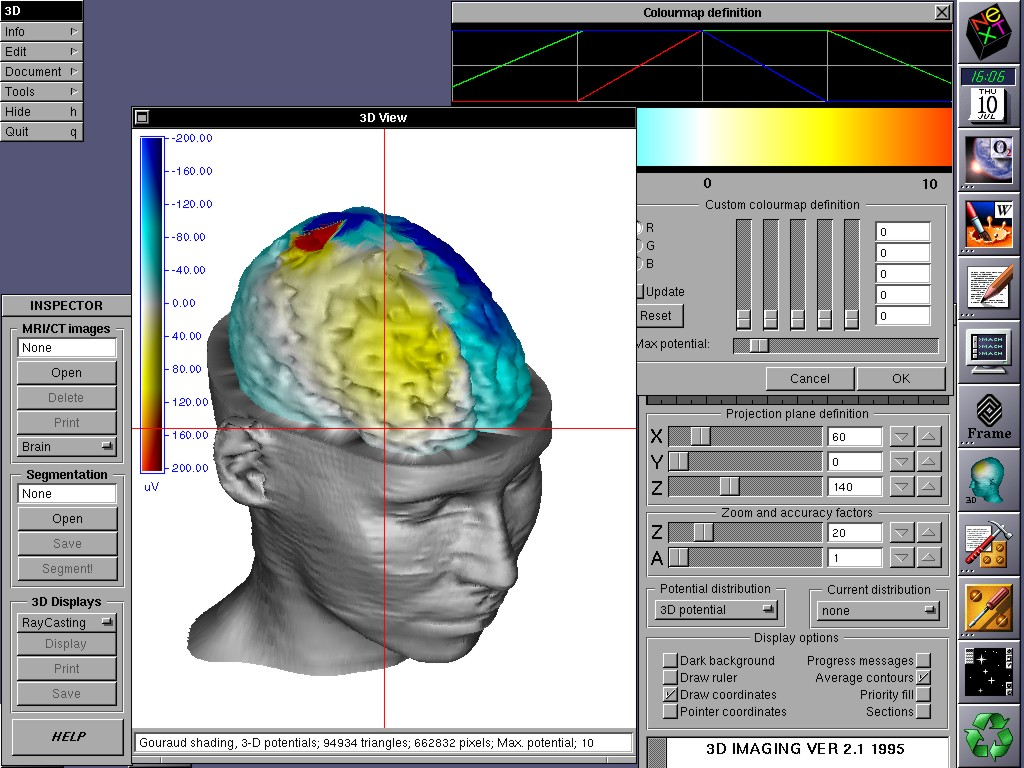
\includegraphics[scale=0.2]{figures/visualizations/medical_visualization.jpg} 
\caption{Example of data visualization in the medical sector.}\label{fig:datavis_medical}
\end{figure}
\begin{remark}
These are \textit{categories} of data visualizations, each category is further subdivided into many more types. Moreover, there are still many (often topic specific) visualizations that we will not touch on (e.g.~medical visualization, see Figure \ref{fig:datavis_medical}). However, in most cases, you will be able to create an appropriate visual using one presented in this work, but you should always remain on the lookout for new \& alternative ways to visualize your data!
\end{remark}

\subsection{Motivation}
In the realm of data science, information is abundant, but knowledge is priceless. Data visualization acts as the brushstroke that brings life to raw data, transforming it into a vivid and intuitive masterpiece. By leveraging the power of visual representation, data visualization enables us to unlock the true potential of our data, making complex concepts more accessible, patterns more discernible, and insights more compelling. In this section, we explore the options one has in visualizing data. As a data scientist/data analyst/machine learning engineer or whichever role in data, we spent days and days exploring data, developing models, testing hypotheses,... We are passionate about this work and appreciate the beauty in being able to predict the total number of passengers on a Boeing 747 with up to $98\%$ accuracy. However, in the end, all our hard work must generate \textit{business value}. In order for this to happen, people must be made aware of our work, its value and applicability. This mostly boils down to having many meetings and presentations where you want to create a mutual understanding of what the data tells us and how this story can help us create business value.

\begin{figure}[htbp]
  \centering
  \begin{minipage}[b]{0.3\textwidth}
    \centering
    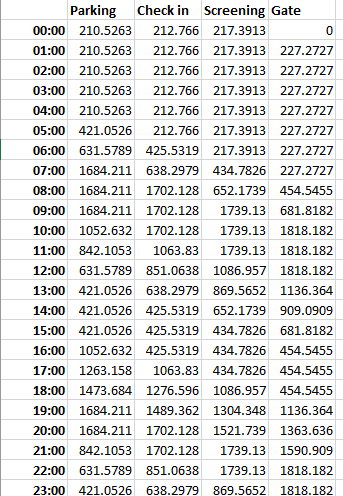
\includegraphics[width=\textwidth]{figures/visualizations/01table.png}
  \end{minipage}
  \hfill
  \begin{minipage}[b]{0.3\textwidth}
    \centering
    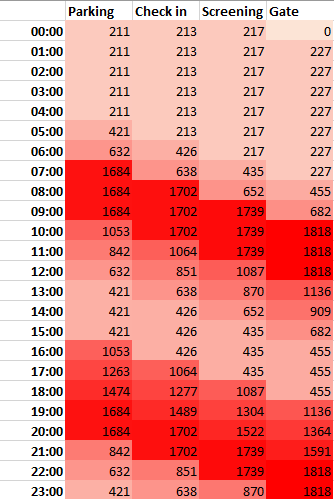
\includegraphics[width=\textwidth]{figures/visualizations/01heatmap.png}
  \end{minipage}
  \caption{We show the number of passengers passing by a number of locations at the airport per 1 hour slot. On the left numbers are shown without and on the right with heatmap.}
  \label{fig:heatmap_example}
\end{figure}

\begin{example}
We often need to create schedules in order to process a certain number of people/things in a day (e.g.~number of passengers at the airport, number of visitors arriving to a theme park, number of orders coming in at Amazon, ...). Let's look at the example of looking at the expected number of passengers at the different locations of an airport. We want to generate a quick overview of these numbers while still displaying all information a decision maker needs. The easiest way to do this is simply by putting all numbers for a specific day into a table, a quick and simple way to make this table easier to read without losing information is to round all numbers to the closest integer and using a heatmap to make high values stand out more.

We clearly observe that there are 2 peaks in number of passengers. Given the data, one could supplement this heatmap with historic information on these peaks and the amount of personnel that was required to handle those peaks. This can then be weighed against the peaks we see in this heatmap.
\end{example}
There are many reasons why data visualization is important, some of them are:
\begin{itemize}
\item \textbf{Clarity in Complexity}:
Data, in its raw form, often appears as an intricate web of numbers, symbols, and patterns. Unveiling its inherent complexity can be a daunting task. However, data visualization rises to the challenge, offering a visual narrative that simplifies the complexity and enhances our understanding. By transforming abstract numbers into intuitive charts, graphs, and infographics, data visualization provides clarity and reveals the underlying story within the data. It enables us to grasp intricate relationships, spot trends, and identify anomalies at a glance, empowering us to make more informed interpretations.
\item \textbf{Insightful Communication}:
Data holds tremendous insights, but these insights are of little value if they remain hidden within spreadsheets and databases. Data visualization acts as a bridge between the data and its audience, facilitating effective communication of information, ideas, and discoveries. By presenting data in visually appealing and interactive formats, it engages the viewer's attention and facilitates a deeper understanding of the underlying message. Whether it's presenting research findings, conveying business metrics, or explaining scientific concepts, data visualization empowers us to communicate complex ideas with clarity, brevity, and impact. There are many meetings in life that could be replaced by a couple of good visualizations.
\item \textbf{Decision-Making Catalyst}:
In a world driven by data, making informed decisions is critical. Data visualization plays a pivotal role in this process by transforming data into actionable insights. By presenting data in visual formats that highlight key trends, comparisons, and patterns, it enables decision-makers to discern relevant information swiftly. Interactive dashboards and real-time visualizations further enhance the decision-making process by providing dynamic and up-to-date views of critical metrics. Whether it's optimizing business strategies, improving operational efficiency, or identifying opportunities, data visualization acts as a catalyst, empowering decision-makers to act with confidence and precision.
\item \textbf{Driving Innovation}:
Innovation thrives on exploration and the ability to perceive connections where others see chaos. Data visualization fuels this spirit of innovation by enabling us to spot patterns, identify gaps, and make creative leaps. By visualizing data from diverse sources and perspectives, it fosters interdisciplinary collaboration, encouraging experts from different domains to contribute their unique insights. Visualization tools, such as network graphs and geographic mapping, unravel hidden relationships and expose untapped opportunities. With data visualization as our guide, we navigate uncharted territories and push the boundaries of what is possible.
\end{itemize}

\subsection{Some general (unwritten) rules in data visualization}
Some golden rules which you should always keep in mind when creating data visualizations.

\begin{itemize}
\item Understand your audience and objectives: Clearly define your target audience and the purpose of the visualization. Understand what insights or messages you want to convey and tailor your visualization accordingly.

\item Choose the appropriate visualization type: Select the visualization type that best suits your data and goals. Consider factors such as the data structure, relationships, and the type of analysis you want to perform.

\item Keep it simple and uncluttered: Avoid visual clutter and unnecessary complexity. Simplify your visualizations by removing irrelevant elements and focusing on the key information. Strive for a clean and minimal design that enhances clarity and readability.

\item Use color strategically: Choose colors purposefully to highlight important information, create visual contrast, and guide the viewer's attention. Maintain consistency and ensure that color choices are accessible and meaningful. Consider color-blindness and use color palettes that accommodate different types of color vision. In general: only add additional colors when you feel like this provides additional information for your audience (otherwise the color is a form of clutter).

\item Ensure appropriate scaling: Set the scale of your visualization appropriately to accurately represent the data. Avoid distorting or misleading interpretations by using appropriate axis scales and starting axes from zero, unless there is a specific reason to do otherwise.

\item Label clearly and provide context: Labels are crucial for conveying information accurately. Clearly label data points, axes, and any relevant components of the visualization. Provide additional context through captions, titles, or annotations to help viewers interpret the data correctly.

\item Use appropriate data order and grouping: Arrange the data in a logical order to facilitate understanding. Group related data together to highlight patterns or comparisons. Consider sorting data based on magnitude, time, or any other relevant factor to support meaningful analysis.

\item Incorporate interactive elements (if applicable): If your visualization is interactive, provide intuitive controls or tooltips that allow users to explore the data and gain deeper insights. Interactivity can enhance engagement and enable users to interact with the visualization according to their specific interests or queries.

\item Validate and iterate: Test your visualization with a sample audience or colleagues to gather feedback and identify areas for improvement. Iterate and refine your visualization based on the feedback received to enhance its effectiveness.
\end{itemize}

\subsection{Statistical charts}
When it comes to displaying statistical charts, one crucial decision is whether to use total numbers or distributional numbers. Both approaches have their merits and can provide valuable insights depending on the context and purpose of the chart. Let's explore each option further.

\begin{figure}
\center
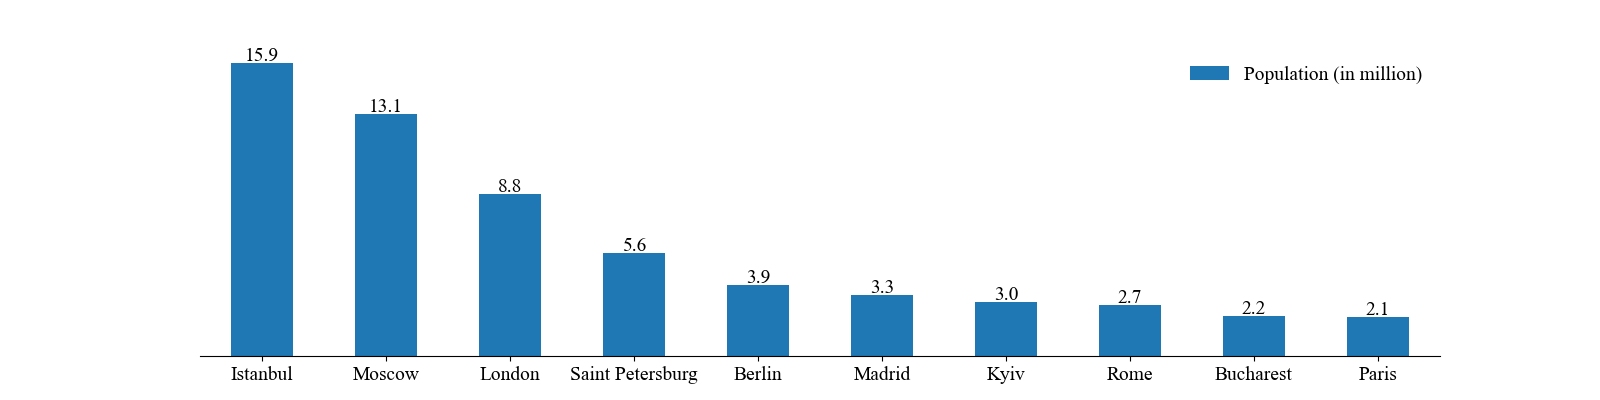
\includegraphics[scale=0.3]{\figuresvisualizationpath/population.png} 
\caption{Example of data visualization in the medical sector.}\label{fig:datavispopulation_cities_bar}
\end{figure}
Using total numbers in statistical charts involves presenting the absolute values or counts of a particular variable. This approach offers a straightforward representation of the data and allows viewers to understand the actual quantities involved. Total numbers are particularly useful when the goal is to convey the magnitude or scale of a phenomenon. For example, if you're comparing the population sizes of different cities, displaying the total numbers can help in easily identifying which cities have larger or smaller populations (see Figure \ref{fig:population_cities_bar}).

\begin{figure}
\center
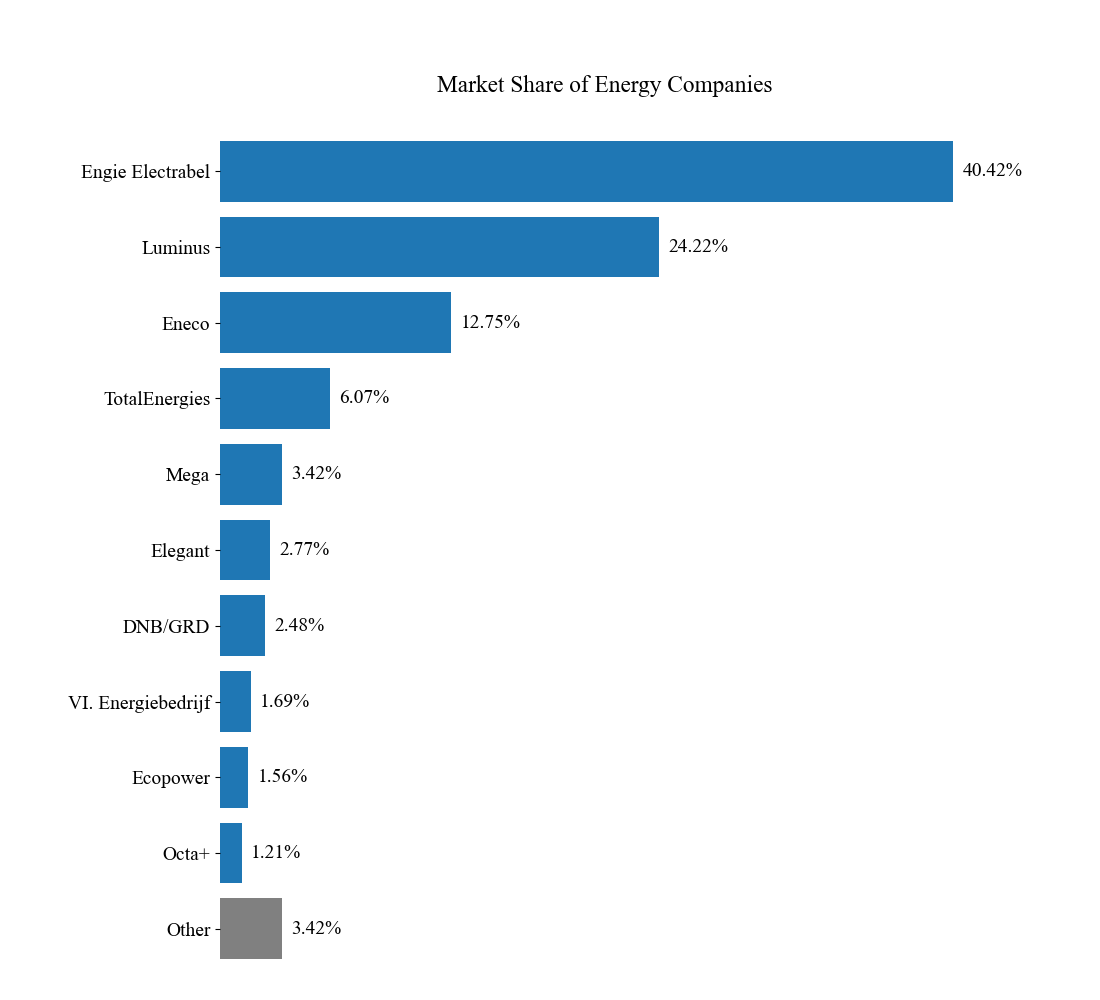
\includegraphics[scale=0.3]{\figuresvisualizationpath/market_shares.png}  
\caption{Example of some data visualization in the energy sector.}\label{fig:datavis_market_shares}
\end{figure}

On the other hand, distributional numbers focus on the proportions or percentages within different categories or groups. Instead of presenting raw counts, this approach highlights the relative distribution of values across the data set. Distributional numbers are valuable when the emphasis is on understanding patterns, trends, or relationships between different groups. For instance, if you're analyzing the market share of various companies within a specific industry, using distributional numbers can reveal the relative dominance or competitiveness of each player. An example of this is show in Figure \ref{fig:population_cities_bar}.

The choice between total numbers and distributional numbers depends on the specific objectives and audience of the statistical chart. If you aim to provide a comprehensive view of the data and prioritize a clear understanding of the overall size or quantity, total numbers may be more appropriate. On the other hand, if your intention is to highlight the relative proportions or share of different components within a dataset, distributional numbers can offer a more insightful representation.

It's worth noting that in many cases, a combination of both approaches can provide a well-rounded depiction of the data. For instance, you can use a chart that presents the total numbers as well as accompanying percentages or proportions within each category. This approach enables viewers to grasp the absolute values while also understanding the relative significance of different groups.

Ultimately, the choice between total numbers and distributional numbers in statistical charts should align with the goals of your analysis and the message you want to convey. By carefully considering the context, audience, and objectives, you can select the most suitable approach to effectively communicate your data-driven insights.

When displaying the values in a distributional sense, you should first be aware of the question whether the distribution your data is coming from is discrete or continuous. Let us first dive into the details on what each type is and how these type of distributions are defined.

\subsubsection{Random variables}
A random variable is a mathematical concept used in probability theory and statistics to represent an uncertain quantity or outcome. It is a variable whose value is determined by the outcome of a random event, such as the roll of a die, the flip of a coin, or the measurement of a physical quantity subject to random variation.

Formally, a random variable is defined as a function that assigns a numerical value to each possible outcome of a random experiment. The set of all possible values that a random variable can take is called its sample space, and the probability distribution of the random variable describes the likelihood of each value occurring.

There are two types of random variables: discrete and continuous.

\subsubsection*{Discrete Random Variables}
A discrete distribution is a probability distribution that describes the probabilities of a random variable taking on specific values. In other words, it represents the likelihood of each possible outcome in a discrete set of values. Unlike continuous distributions, which can take on any value within a range, discrete distributions have a countable set of possible outcomes. These values can either be categorical (such as companies, gender, ...) or discrete numbers (such as the number of eyes on a die, daily production of smartphones, ...). These distributions are defined by assigning a probability to each possible outcome.

\remark{In the example of Figure \ref{fig:population_cities_bar}, one could argue that the random variable we are looking at is \textit{total population} and it takes on the given values for the different cities. Alternatively, if we were only interested in the population of Madrid, we could define our random variable as the population of Madrid and the value of 3.3 million is one observation from this value at a specific point in time. We could then argue that it might be of interest to visualize this total value as a function of time and look at that distribution.}

\subsubsection*{Continuous Random Variables}
A continuous random variable can take any value within a certain range or interval. For example, the height of a person, the time it takes for a car to travel a certain distance and the market share of Engie at different points in time are continuous random variables.

\subsubsection{Bar charts}
Bar charts are commonly used for visualizing categorical or discrete data and displaying comparisons between different categories or groups. They are particularly effective in representing data that can be organized into distinct categories or groups, such as survey responses, sales figures, population distribution, and frequency counts.

Here are some common uses of bar charts:
\begin{itemize}
\item \textbf{Data Comparison}: Bar charts are ideal for comparing the values or frequencies of different categories. The length of each bar represents the quantity or magnitude of the variable being measured, allowing for easy visual comparison. This makes bar charts useful for analyzing data trends, identifying patterns, and drawing insights.

\item \textbf{Data Distribution}: Bar charts can show the distribution of data across categories or groups. Each category is represented by a separate bar, and the height of the bar indicates the frequency, count, or proportion associated with that category. This helps in understanding the distributional characteristics of the data.

\item \textbf{Data Representation}: Bar charts provide a clear and concise way to present data to an audience. They are easy to understand and interpret, making them suitable for conveying information in presentations, reports, and publications.

\item \textbf{Data Exploration}: Bar charts can be used as an exploratory tool to identify patterns, outliers, or anomalies in the data. By visualizing the data in a bar chart, you can quickly spot variations or discrepancies between different categories, which may lead to further investigation or analysis.

\item \textbf{Data Comparison over Time}: Bar charts can also be used to compare data across different time periods. By arranging bars chronologically, you can observe changes or trends in the data over time. This is particularly useful for tracking progress, analyzing historical data, or identifying seasonal patterns.
\end{itemize}

Overall, bar charts provide a simple and effective way to display and analyze categorical data, making them a popular choice for data visualization and communication purposes. As such, a number of different types of bar charts have been developed. Some general tips to keep in mind when creating a bar chart:
\begin{itemize}
\item Choose appropriate colors: It's recommended to use the same colors for similar categories while using contrasting colors between sufficiently different categories. Avoid using colors that may convey unintended meaning or bias. In the example of Figure \ref{fig:datavis_market_shares}, we used a single color for all actual companies and we \textit{greyed out} the \textquotedblleft Other\textquotedblright  category.

\item Maintain a logical data order: Arrange the bars in a logical and meaningful order to facilitate easy comprehension. Typically, it is best to sort the categories in ascending or descending order based on the variable being measured. This helps in identifying patterns, trends, or outliers more effectively.

\item Avoid excessive clutter: Keep the design clean and uncluttered by removing unnecessary elements that may distract or confuse viewers. Minimize gridlines, borders, or background patterns if they do not add value to the chart. Focus on presenting the data in a clear and straightforward manner.

\item Use appropriate scales: Ensure that the scale of the axes is appropriate for the data being represented. Avoid distorting the perception of data by using uneven or misleading scales. Start the y-axis (vertical axis) from zero unless there is a specific reason to use a different baseline.
\end{itemize}

\subsubsection*{Vertical bar charts}
This is the most common type of bar chart, where the bars are displayed vertically along the y-axis. Each bar represents a category or group, and the length of the bar corresponds to the value or frequency associated with that category. Vertical bar charts are useful for comparing data across different categories or groups. We already had an example of this type of bar charts in Figure \ref{fig:datavispopulation_cities_bar}. Some things to keep in mind when creating this type of bar chart

\subsubsection{Horizontal bar charts}
In a horizontal bar chart, the bars are displayed horizontally along the x-axis. Like vertical bar charts, each bar represents a category or group, and the length of the bar indicates the value or frequency. Horizontal bar charts are often used when the category labels are long or when there are many categories to display.

\subsubsection{Grouped bar charts}
A grouped bar chart displays multiple sets of bars side by side, allowing for easy comparison between different groups. Each group represents a category, and within each group, there can be multiple bars representing subcategories or different variables. Grouped bar charts are useful for comparing values across multiple categories simultaneously. These can of course be either vertical or horizontal.

\subsubsection{Stacked bar charts}
In a stacked bar chart, the bars are stacked on top of each other, with each segment of the bar representing a subcategory or component. The total height of the bar represents the cumulative value or frequency of all the subcategories. Stacked bar charts are suitable for showing the composition or breakdown of a variable across different categories.

\subsubsection{$100\%$ stacked bar charts}
Similar to a stacked bar chart, a $100\%$ stacked bar chart also displays bars stacked on top of each other. However, the height of each bar is normalized to represent the relative proportion or percentage of each subcategory within the total. This type of chart is useful for comparing the relative contribution of different subcategories across categories.

\subsubsection{Clustered bar charts}
A clustered bar chart displays bars grouped together in clusters, with each cluster representing a category. Within each cluster, there can be multiple bars representing different variables or subcategories. Clustered bar charts are suitable for comparing values between different categories and within each category.

\section{Statistics for Data Science}
\todo{Insert drawings to explain math in data science and the whole pipeline pointing at where you use which math/skills.}
Thus far, we have mainly focused on the technical skills that allow you to work with data, this includes:
\begin{itemize}
\item Basic python to think programmatically (if/for/while loops, variables, errors, \dots). 
\item We zoomed in on the python you need to work with data specifically; this includes working with files/folders on your computer but also to connect to an external database, scrape information from a website etc..
\item We then focused on tabular data, this is mainly done with Pandas, a python package which allows you to quickly combine data from multiple tables and process data in a table.
\item We also looked at numpy which contains functionality specifically to work with tensor data, these include 1 dimensional \textit{vectors}, but also 2 dimensional \textit{matrices} and we also looked at three dimensional tensors in the form of RGB images.
\end{itemize}
This chapter concludes the more technical part of the course and from here on out, in this second part of the course, we are going to focus more on the conceptual side and less on the technical. We will still have many exercises in Python and you are still expected to be able to \textquotedblleft do\textquotedblright  everything we discuss in Python (or any other programming language) but the technical implementation will no longer be the focal point. We start this chapter by providing an overview of the position of math in the data scientist's workflow. 

In the subsequent sections, we introduce basic statistics that lie at the heart of data science. These contain fundamentals of statistics (such as the definition of a probability density function, how to visualize probability distributions etc.), but also some classical statistics results that are often (mis)used in the real world. One of the most important results in statistics is the central limit theorem. This theorem is often interpreted as \textit{you can model any reasonable random variable as a normal distribution}, but this is not at all the case! Simply being able to spot when the normal distribution is being misused can already add a lot of value to a company (see also section \todo{ref naar sectie CLT}).

\subsection{Required math for data science}
For many aspiring data scientists, a good foundation in math may seem daunting. However, when starting to learn data science/machine learning, it is not necessary to immediately delve into learning all aspects of mathematics. While mathematics plays a fundamental role in understanding the underlying concepts of machine learning, it can be overwhelming to tackle all math topics at once. A few reasons why you shouldn't start with learning all math for data science are:

\begin{enumerate}
\item \textbf{Steep learning curve}: Mathematics can be complex, and diving into advanced topics without a solid foundation can make it difficult to grasp the concepts. It's better to approach mathematics progressively, starting with the basics and gradually building up your knowledge as you gain more experience with machine learning.

\item \textbf{Practicality}: Machine learning frameworks and libraries provide high-level abstractions that allow practitioners to apply machine learning techniques without extensive mathematical knowledge. These tools offer pre-implemented algorithms and functions, making it easier to get started and achieve meaningful results without delving into the underlying mathematics.

\item \textbf{Focus on application}: Initially, it's more important to understand the practical aspects of machine learning, such as data preprocessing, model selection, and evaluation. By focusing on these areas, you can gain hands-on experience and develop intuition about how machine learning works in real-world scenarios.

\item \textbf{Learning by doing}: Machine learning is a highly practical field. Engaging in projects and implementing machine learning algorithms will help you understand the core concepts and their mathematical underpinnings more effectively. This hands-on approach will allow you to see the direct application of mathematics in machine learning.
\end{enumerate}

\begin{remark}
The approach we will be taking is the learning by doing, that is, we provide the math required as we come across it. Moreover, this explanation will be on the intuition rather than arithmetics. For example:

When someone asks you to compute $\int_8^12 \sin(x) \cdot x^2 \, dx$ and \textit{explain} how you did it, I do not expect you to be able to take out pen and paper and be able to exactly compute this integral. You should be able to (with the help of google) use Python to compute this value through the function \texttt{np.trapz}. Ideally, you should also be able to plot the function $f(x) = \sin(x) \cdot x^2$ and explain that the area under the curve on the interval $[8,12]$ corresponds to the integral that this person is inquiring about (see also Figure \ref{fig6.1:integral}). Ideally, you would also be able to explain how this integral comes into existence as the limit of the surface area of histograms with an increasing number of bins.
\end{remark}

\begin{figure}
\begin{center}
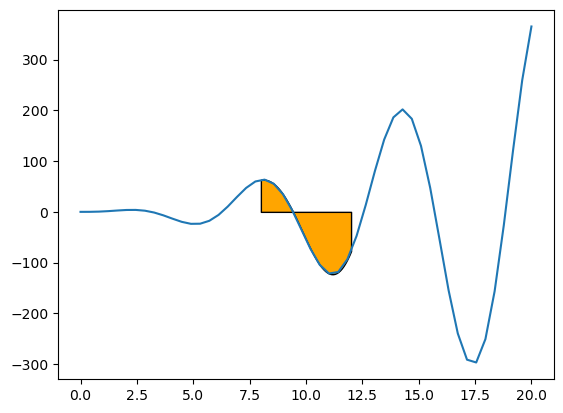
\includegraphics[scale=0.4]{figures/6.1_integral.png}
\caption{Integral $\int_8^12 \sin(x) \cdot x^2 \, dx$ visualized.} \label{fig6.1:integral}
\end{center}
\end{figure}

The part of Data Science for which one requires the most math is typically when developing a machine learning model. Typical projects consist of (a selection from) the following steps:
\begin{enumerate}
\item Collect the data from different sources (no math).
\item Merge and clean the data from all sources into a compatible format (almost no math).
\item Slice, dice and preprocess the data to be ready to be fed into some statistical tool (e.g.~a machine learning algorithm). This mostly requires some linear algebra which is the mathematical field of doing computations on tensors.
\item Explore the data using standard data analysis tools (requires some probability/statistics knowledge).
\item Select and execute an appropriate method to tackle the given problem. Here the underlying probability theory can be regarded as the beating heart of the method. In order to understand what you are doing and what results you are getting, you will always need a basic level of probability/statistical knowledge. In order to truly understand what is happening under the hood, you will need a lot of deep probability theory knowledge. This should not be your goal at this point.
\item Calculus and optimization come into play when we have selected a model and we now want to train our model, that is we want to tweak our conceptual model to our specific case. This means that we want to find the \textit{optimal} parameters for our problem setting and this in turn requires some basic understanding of calculus and optimization theory in order to \textit{kind of} know what you are doing and deep knowledge of these subjects to truly understand it (which, again, is not the goal at this point in time).
\end{enumerate}
\begin{remark}
In Sections \ref{sec:linreg} and \ref{sec:grad_desc}, we will look at our first machine learning algorithm and give a high level overview of how the above process plays out for linear regression. 
\end{remark}
We now start this chapter by first looking at the basics of (applied) statistics and look at some of the most important results in statistics. The reason why we start our quest here is three-fold:
\begin{enumerate}
\item Nowadays, it is a popular belief that Machine Learning is the only method that can be used to solve problems using data. This belief is however completely bogus, for many problems, simple statistics are sufficient.
\item An algorithm is often used to create predictions, these predictions are by definition uncertain. Therefore having a sense of how to talk about uncertainty is required in order to talk about predicting.
\item A basis in statistics is quite standard in many school curricula, therefore this content will be somewhat familiar to many people. However, due to this \textit{somewhat familiarity}, the results are often used in an incorrect way leading to illogical decisions. Using a combination of data visualizations and statistical knowledge these mistakes can often be laid bare and the search for a more sensible methodology can be sought.
\end{enumerate}
\begin{remark}
The field of solving problems using data is of course much broader than statistics or machine learning. There's also Operations Research, graph algorithms and simulations, just to name a few alternative methods. Which methodology should be used is highly dependent on the problem at hand and it is always an important decision to select the right framework for a given problem.
\end{remark}
Without further ado, let us dive into an overview of the types of data one may encounter.
\subsection{Types of data}
\todo{Section describing all types of structured data}

\subsection{Estimating center locations}
\todo{Section describing types of center locations and when to use which.}

\subsection{Variability}

\subsection{Exploring distributions \& Bayes Theorem}
In this section we talk 

\subsection{Linear Regression \& the standard ML flow} \label{sec:linreg}
In previous section, we learned about conditional probabilities and Bayes theorem. Conditional probabilities lie at the heart of (almost) all machine learning problems, we constantly ask ourselves questions like:
\begin{itemize}
\item What should the prize of a house be given its surface area, location, \dots
\item What is the probability of being a survivor on the titanic given your age, gender, \dots
\item Etc.
\end{itemize}
Before we dive deeper into the \textit{statistical} approach of solving these type of questions, let us look into the most taught machine learning method in existence: \textit{Linear Regression}.

We are given a dataset consisting of the medical costs for a group of 1339 Americans. For these people, we are given the age, sex, bmi (body mass index), number of childen, whether they smoke, the region they live in and the total amount of medical charges they have been charged in their life.

\begin{figure}
\begin{center}
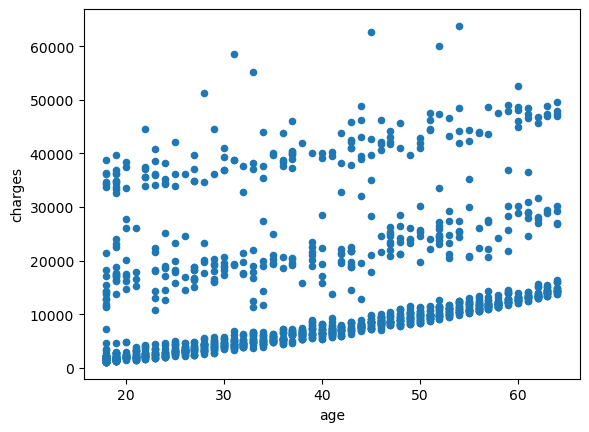
\includegraphics[scale=0.4]{figures/6.5_linear_regression.png}
\caption{Scatterplot comparing the total medical cost of a person with his age.} \label{fig:6.5_linear_regression}
\end{center}
\end{figure}

Let us start by focusing on linear regression with only one feature, we expect a person's age to be the most telling, therefore we will try to predict the a person's medical cost solely based on his age. Therefore age is the input feature and the medical cost is the target or dependent variable. We can visualize the relation between the two features using a scatterplot, see Figure \ref{fig:6.5_linear_regression}.
\begin{remark}
From this scatterplot, we can immediately see that there clearly is some connection between age and medical cost, but that we still require some additional information in order to split the dataset further. For ease of notation we will nonetheless first focus on the case with only one input feature (age), but afterwards we will investigate how we can effectively use multiple features in order to more accurately predict the medical charges.
\end{remark}
We have chosen for linear regression with only one feature, therefore our model looks like:
\begin{equation}\label{eq:linreg_1feature}
h(x) = \theta_0 + \theta_1 \cdot x,
\end{equation}
that is a straight line that passes through the $y-axis$ at $\theta_0$, we call $\theta_0$ the intercept. It then linearly increases linearly with a slope equal to $\theta_1$. We are now looking for a \textit{optimal} values for $\theta_0$ and $\theta_1$ such that the line defined by $y=h(x)$ fits the distribution of points in Figure \ref{fig:6.5_linear_regression} as closely as possible.

To this end, we first need to quantify the error made by a prediction, this is done by defining a loss function $\ell(x)$. The most typical loss function used for linear regression is the Root Mean Squared Error (or RMSE in short), it is defined by:
\begin{equation} \label{eq:RMSE}
\ell_{\theta}(x) = \sqrt{ \frac{1}{n} \sum_{i=1}^n \frac{(h(x_i) - y_i)^2}{n} }.
\end{equation}
Here, we denote by $n$ the total number of samples, by $x_i$ the age of sample $i$ and by $y_i$ the actual medical costs charged to the sample.
\begin{remark}
This loss function in \eqref{eq:RMSE} (referred to as the RMSE) can alternatively be written as:
\begin{equation} \label{eq:RMSE_yhat}
\ell(x) = \sqrt{ \frac{1}{n} \sum_{i=1}^n \frac{(\hat{y}_i - y_i)^2}{n} },
\end{equation}
with $\hat{y}_i = h(x_i)$, the prediction for sample $i$. Using this notation one can clearly see that this is a general formula which can be used to measure the performance of any model.
\end{remark}
\begin{remark}
There is a strong resemblance between the RMSE and the standard deviation! If we would use the average of all $y_i$ as prediction, we find that \eqref{eq:RMSE_yhat} is exactly the variance of the sample data $(y_i)_i$. This \textit{mean estimate} is often used as a base case and any model that you use can be seen as improving this base case, that is: predicting (a part of) the variability in the distribution $(y_i)_i$.
\end{remark}

In the loss function in \label{eq:RMSE_yhat} we have $x_i$, $y_i$ and $n$ which are fixed given the dataset. We can however still determine the values of $\theta_0$ and $\theta_1$ in order to find a good fit. We can therefore visualize $\ell_{\theta}(x)$ as a function of $\theta_0$ and $\theta_1$. We
\begin{figure}
\begin{center}
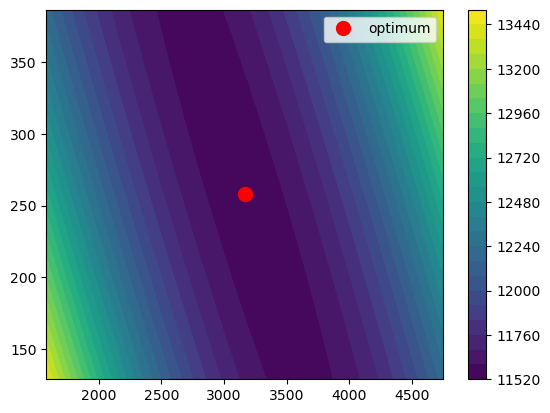
\includegraphics[scale=0.8]{figures/6.5_error_fun.png}
\caption{The loss function in \eqref{eq:RMSE} visualized for the medical charges example visualized.} \label{6.5_error_fun.png}
\end{center}
\end{figure}

\subsection{Gradient descent} \label{sec:grad_desc}

\end{document}